\section*{Assignment 02: Network Effects and Launch Strategy}
\addcontentsline{toc}{section}{Assignment 02: Network Effects and Launch Strategy}

\subsection*{Network effects mapped explicitly}
I followed \citet{Choudary2016}'s three step loop mapping exercise to keep the network effects honest. Step one defines the core interaction: a vetted organisation posts a scoped brief, curated students respond, and both sides commit to a sprint. Step two specifies reinforcing signals. The cross side loop grows when visible success stories and quick responses reassure the next wave of users. Student same side effects stem from peer endorsements and a ritual where alumni leave short Loom videos once a sprint ends, echoing Lecture~4's point that social proof reduces cold start friction \citep{Lecture04}. Organisation same side effects emerge when NGOs see comparable peers succeeding, so I pencilled monthly showcase calls. Finally the data loop records skills used, hours invested, and satisfaction scores, upgrading the matching algorithm each cycle and nudging SkillSync toward the curated orchestrator pattern \citep{Reillier2017}.

\subsection*{Solving the penguin problem}
To break the mutual hesitation \citet{HagiuWright2013} warn about, the launch plan recruits two anchor NGOs already comfortable mentoring students. They become the first proof points and agree to share testimonials. Parallel to that, I recruit a founding cohort of forty students through faculty recommendations, student societies, and the course Slack so quality stays predictable. A concierge onboarding script walks both sides through the first mission: I manually review briefs, pair mentors, and host a kickoff call. Subsidies stay targeted. Students receive travel stipends for the first sprint funded by a faculty innovation grant, while NGOs get a temporary fee waiver that expires after two successful projects, following \citet{FarrellSaloner1986}'s logic on introductory pricing.

Communication routines are scripted in advance. Weekly check ins and a shared calendar keep the first ten projects on track; we log every friction point and feed it into a public FAQ. The cadence mirrors Lecture~4 guidance: when seeding a platform, design commitment devices that keep early adopters active long enough for loops to form \citep{Lecture04}. I also plan a backup: if a project fails mid sprint, SkillSync deploys a standby student pair from the founding cohort within forty eight hours, so organisations trust us despite hiccups.

\subsection*{Launch measurements and decision rules}
Because there is no live product yet, my reflections read like a pre mortem. I focus on three metrics. Time to first value measures minutes from signup to first concrete action; if it exceeds thirty minutes the concierge team must simplify the brief wizard. Match completion rate tracks how many pairs finish within scope; a dip below seventy percent triggers a root cause session. Early net promoter score captures qualitative trust; scores below plus twenty prompt follow up interviews. These numbers come from \citet{ShapiroVarian1999}'s advice to anchor monetisation on observed value and from Lecture~5's insistence that early experiments should move one behaviour at a time \citep{Lecture05}. Figure~\ref{fig:application-flow} visualises the guided student flow that underpins these metrics.

\begin{figure}[H]
  \centering
  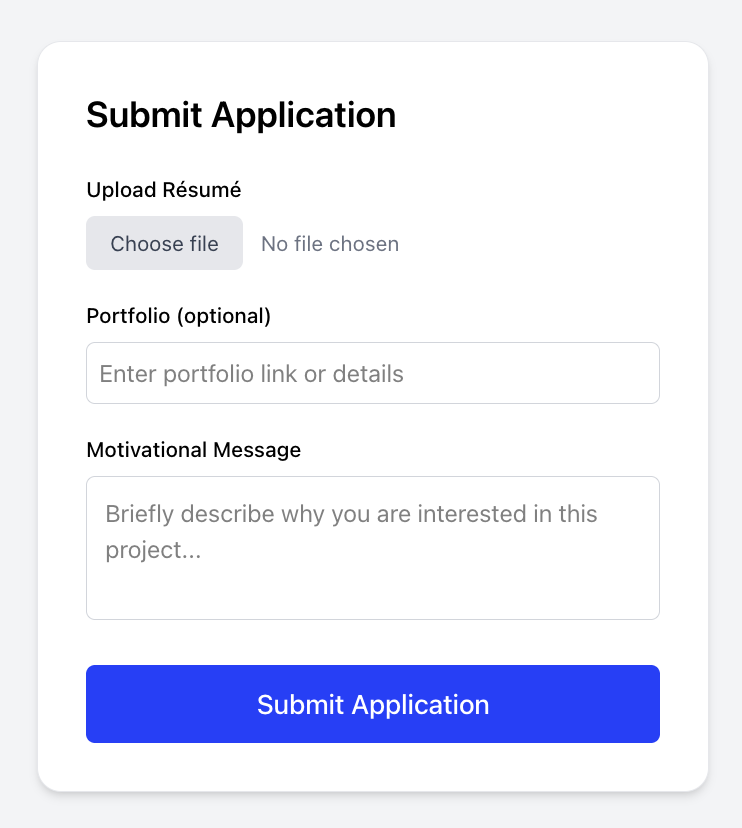
\includegraphics[width=0.85\linewidth]{figures/Student-Submission.png}
  \caption{Student application flow mock up with guided pitch submission.}
  \label{fig:application-flow}
\end{figure}

I mirror the journey for organisations in Assignment~03. The idea is to choreograph both sides simultaneously so that once the early subsidies phase out, the playbook already embeds trust and rhythm instead of improvising fixes.
